\documentclass[tikz, border=1mm]{standalone}

%Packages
\usepackage{xcolor} %Advanced colors
\usepackage{pgfmath} % Advanced calculus

%Pallet colors
\definecolor{spinUP}{HTML}{181818}
\colorlet{spinDOWN}{white}
\definecolor{j1}{HTML}{535FA6}
\definecolor{j2}{HTML}{247373}
\definecolor{j3}{HTML}{F2A74B}
\definecolor{j4}{HTML}{A63B32}

%Parameters
%size lattice
\newcommand{\Lx}{3} %horizontal
\newcommand{\Ly}{3} %vertical
\newcommand{\LL}{3} %square
\newcommand{\lw}{1} %line width
\newcommand{\ptTOcm}{1./28.45274} %convert pt to cm
\pgfmathsetmacro{\burr}{0.5*\lw*\ptTOcm}

%Spins(circles)
\newcommand{\sizeCircle}{0.15}
\newcommand{\povGlow}{280}

\begin{document}
	%%%%%%%%%%%
% Loop and grid 
% M. Roos, 10/11/2024
%%%%%%%%%%%

% Square lattice (Lx = Ly = LL) - 1 loop above vertical and horizontal lines
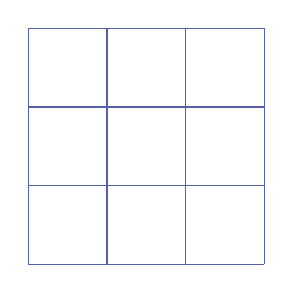
\begin{tikzpicture}
	\foreach \i in {0,1,...,\LL}{
		\draw[j1] (\i,0) -- (\i, \LL); %horizontal
		\draw[j1] (0,\i) -- (\LL, \i); %vertical
	}
\end{tikzpicture}

% Within loop, use grid, since (x0, y0) at (Lx, Ly)
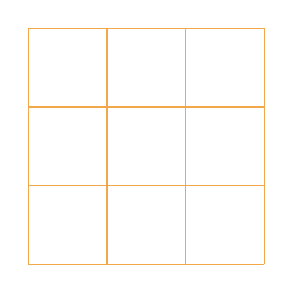
\begin{tikzpicture}
	\draw[j3, step=1cm] (0,0) grid (\LL, \LL);
\end{tikzpicture}

% Resolve burr
\begin{tikzpicture}
	\node at (0.5,0.4) {1cm = 28.45274pt};
	\draw[j4, line width=\lw] (0,0) -- (1,0);
	\draw[red, line width=\lw] (0.5,0 -\burr ) -- (0.5, \burr);
\end{tikzpicture}

% Grid within burr
\begin{tikzpicture}
	\foreach \i in {0,1,...,\LL}{
		\draw[j4, line width=\lw] (\i,0) -- (\i, \LL);
		\draw[j4, line width=\lw] (0 - \burr,\i) -- (\LL + \burr, \i);
	}
\end{tikzpicture}

% Grid with spins (circles)
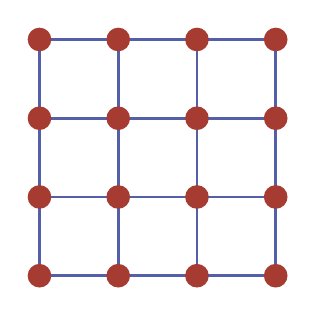
\begin{tikzpicture}
	\draw[j1, step=1cm, line width=1] (0,0) grid (\LL, \LL);
	\foreach \j in {0,1,...,\LL}{
		\foreach \i in {0,1,...,\LL}{
			\fill[j4] (\i,\j) circle(\sizeCircle) ; 
		}
	}
\end{tikzpicture}

% Circles with shadow and glow
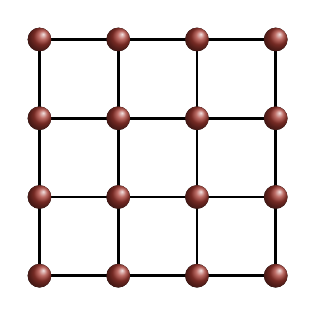
\begin{tikzpicture}
	\draw[step=1cm, line width=1] (0,0) grid (\LL, \LL);
	\foreach \j in {0,1,...,\LL}{
		\foreach \i in {0,1,...,\LL}{
			\fill[ball color=j4, shading angle=\povGlow] (\i,\j) circle(\sizeCircle) ; 
		}
	}
\end{tikzpicture}

\end{document}